% !TeX program = pdflatex
\documentclass[tikz,border=8pt]{standalone}
\usepackage{tikz}
\usetikzlibrary{positioning}
\definecolor{FigureBlue}{HTML}{2563EB}
\definecolor{FigureGreen}{HTML}{16A34A}
\definecolor{FigureOrange}{HTML}{EA580C}
\definecolor{FigureSlate}{HTML}{64748B}
\begin{document}
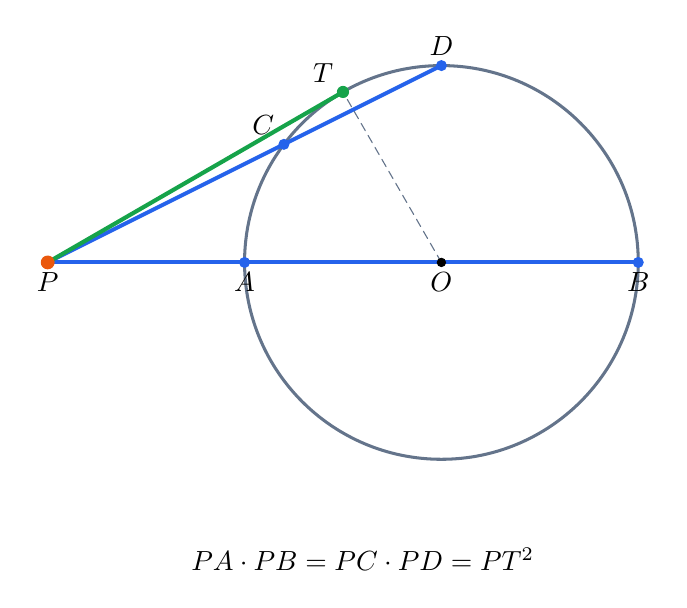
\begin{tikzpicture}[line cap=round,line join=round]
  \coordinate (O) at (1,0);\coordinate (P) at (-4,0);
  \coordinate (A) at (-1.5,0);\coordinate (B) at (3.5,0);
  \coordinate (C) at (-1,1.5);\coordinate (D) at (1,2.5);
  \coordinate (T) at (-.25,2.1650635);
  \draw[FigureSlate,line width=1.1pt] (O) circle[radius=2.5];
  \draw[FigureBlue,line width=1.4pt] (P)--(B);
  \draw[FigureBlue,line width=1.4pt] (P)--(D);
  \draw[FigureGreen,line width=1.5pt] (P)--(T);
  \draw[FigureSlate,densely dashed] (O)--(T);
  \foreach \P in {A,B,C,D}{\fill[FigureBlue] (\P) circle (2pt);}
  \fill[FigureGreen] (T) circle (2.2pt);\fill[FigureOrange] (P) circle (2.5pt);\fill (O) circle (1.7pt);
  \node[below] at (P) {$P$};\node[below] at (A) {$A$};\node[below] at (B) {$B$};
  \node[above left] at (C) {$C$};\node[above] at (D) {$D$};\node[above left] at (T) {$T$};\node[below] at (O) {$O$};
  \node[below=10mm] at (0,-2.5) {$PA\cdot PB=PC\cdot PD=PT^2$};
\end{tikzpicture}
\end{document}
